
\chapter{Real Numbers}

The calculus depends on a system of numbers.  They are called ``the
continuum'', ``the real numbers'', or simply ``the reals''.  Geometry provides
a way to visualize the reals: Imagine a straight line and associate a different
number with every point on the line, so that the numbers increase in one
direction and decrease in the opposite direction. See
Figure~\ref{fig:number-line}, which illustrates a \emph{real number line} or a
\emph{coordinate line}.  For every \emph{displacement} from the origin, there
is a corresponding real number, which may be rational\footnote{%
   Equal to the ratio of two integers. The decimal representation of every
   rational number, like $\frac{1}{2} = 0.5 = 0.5\bar{0}$, repeats. Between
   every two distinct points on the number line, no matter how close together
   they are, there is an infinite number of rationals. So one might imagine
   that every point on the number line corresponds to a rational number.
   However, at least so far back as the Fourth Century, B.C., Greek
   mathematicians were aware that $\sqrt{2}$ is not rational. Despite the fact
   that the rationals are everywhere dense on the number line, there are also
   irrationals on the number line.
},
irrational\footnote{%
   Not equal to the ratio of two integers. The decimal representation of an
   irrational number, like $0.21221222122221\ldots$, never repeats and, like
   the decimal representation of $\pi = 3.14159265358979\ldots$, might not have
   an obvious pattern.%
}, or even non-computable\footnote{%
   A \emph{non}-computable number has no algorithm that can be used to
   calculate its value so precisely as desired.  Every irrational number (like
   $\sqrt{2}$ or $\pi$) that is used as an example in ordinary algebra,
   geometry, or calculus is a \emph{computable number}.  Among the computables
   are only every real number whose value can be approximated, by way of some
   algorithm, to arbitrary precision.  On the one hand, because the set of
   algorithms is \emph{countably} infinite, the set of computables is also
   countably infinite. On the other hand, the set of reals is
   \emph{un}countably infinite because, as Cantor proved in 1874 and in a
   different way in 1891, there exists no bijection between the natural numbers
   and the real numbers.
   
   In his {\it Shadows of the Mind: A Search for the Missing Science of
   Consciousness}, Roger Penrose provides a good discussion of what an
   algorithm is and why the strange non-computables lead to the uncountability
   of the reals.%
}. The calculus refers to the \emph{limit} of a sequence of numbers, and, even
if every member of a sequence be rational, the limit of the sequence might be
irrational or non-computable.\footnote{%
   Consider the sequence, $(0.21, 0.21221, 0.212212221, \ldots)$.  Every member
   of the sequence is rational, but the limit of the sequence is irrational. In
   this example, the limit is computable.  There has been some interesting work
   on determining how much of the calculus can be retained on the replacement
   of the reals with the computables.%
}
The set of real numbers contains every limit required by the calculus.

The name ``real'' was introduced in the 1600s by Ren\'e Descartes.\footnote{%
   Descartes was a mathematician and a philosopher. His contribution to
   mathematics is substantial.  However, we view his departure from the
   hylemorphic metaphysics of Aristotle and St.~Thomas Aquinas as a crucial
   error in the history of philosophy. For a good introduction to the
   hylemorphism, see {\it Aquinas: A Beginner's Guide\/} by Edward Feser.
}
Descartes distinguished the \emph{real} square root of a positive number from
the \emph{imaginary} square root of a negative number. As Newton later did
explicitly, Descartes implicitly treated every real number as the ratio of a
length to a unit length.\footnote{%
   According to the encyclopedia entry on Descartes at {\scriptsize
   \texttt{thefreedictionary.com}}, ``Descartes treated a real number as the
   ratio of any line segment to the unit segment, although such a definition
   for real numbers was explicitly stated much later by I. Newton; negative
   numbers were given a real interpretation in Descartes's work as directed
   ordinates.''%
}
The ancient Greeks, too, thought of number in terms of length. We shall develop
the reals in a way that reflects this ancient tradition of regarding a number
as a ratio of lengths.

The set of real numbers is denoted by the symbol ``$\mathbb{R}$''.  We take the
idea of displacement to be more fundamental than distance, and we introduce the
idea of a dimensioned quantity, in which a fundamentally geometric unit is
scaled by a real number.  Considering the ideas of order and distance, we
introduce the idea of open and closed intervals on $\mathbb{R}$.  The
development of some basic intuition about $\mathbb{R}$ prepares us for the
discussion of the limit.

\begin{figure}
   \begin{center}
      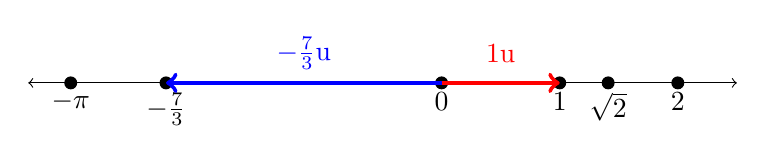
\begin{tikzpicture}[scale=1.5]
         \draw[<->] (-3.5,0) -- (2.5,0);
         \filldraw (-3.14,0) circle [radius=0.05] node[anchor=north] {$-\pi$};
         \filldraw (-7.0/3.0,0) circle [radius=0.05] node[anchor=north]
         {$-\frac{7}{3}$};
         \filldraw (0,0) circle [radius=0.05] node[anchor=north] {$0$};
         \filldraw (1,0) circle [radius=0.05] node[anchor=north] {$1$};
         \filldraw (2,0) circle [radius=0.05] node[anchor=north] {$2$};
         \filldraw (1.41,0) circle [radius=0.05] node[anchor=north]
         {$\sqrt{2}$};
         \draw[->,ultra thick,red] (0,0) -- (1,0);
         \draw[->,ultra thick,blue] (0,0) -- (-7.0/3.0,0);
         \draw (0.5,0.25) node[red] {$1\mathrm{u}$};
         \draw (-3.5/3.0,0.25) node[blue] {$-\frac{7}{3} \mathrm{u}$};
   \end{tikzpicture}
\end{center}
   \caption{A Cartesian coordinate system on a line allows one to visualize
      every real number $r$ as the coordinate of a point. The coordinate gives
      the point's displacement from the origin, whose coordinate is~$0$. A
      displacement is not merely a distance but a directed distance. The unit
      $\mathrm{u}$ of displacement is the directed distance from the origin to
      the point whose coordinate is~$1$.%
   }
\label{fig:number-line}
\end{figure}

\section{Coordinate}

The real numbers are not simply the elements of the set $\mathbb{R}$; each real
number is related to every other real number in certain, well defined ways. For
any two distinct real numbers, one is \emph{greater than} the other, and so the
reals are ordered.  Also, for any two real numbers, there is a distance between
them, and so $\mathbb{R}$ is a \emph{metric space}.\footnote{%
   A metric space is a space of measurement. The idea is that we can, at least
   in an abstract sense, \emph{measure} the distance between any two elements
   of the space.%
}
In their ordered and metric nature, the reals are more than just a set of
elements.

Some of the structure of the reals can be exposed by way of geometry; we can
identify a deep correspondence between geometry and number.  Recall
Figure~\ref{fig:number-line}, which depicts the coordinate line.  Considering
order and distance together, we may define for any two distinct real numbers a
\emph{displacement}, the directed distance from the first to the second.
Because the first is either less than or greater than the second, the
displacement is either \emph{positive} or \emph{negative} in its direction.
Noting the similarity between the coordinate line and a ruler, we use the
coordinate line to visualize the nature given to $\mathbb{R}$ by ordinary
arithmetic operations and comparisons.

\subsection{Displacement}

An abstract geometric displacement, which has both a length and a direction, is
an example of a \emph{vector}. In the one-dimensional metric space of a line, a
symbol like ``$v$'', representing any vector, has no special notation to
distinguish it from a symbol representing a number. (We shall in a later
chapter see that in a two-dimensional or higher-dimensional space, the symbol
for a vector will appear as ``$\vec{v}\:$''.) Although it can be
scaled---multiplied---by a number, a displacement is not itself a number.
Whenever we establish a fundamental unit of displacement, in terms of which
most or all other displacements are expressed, we represent this unit without
italics, with a symbol like ``$\mathrm{u}$''. Thus we might write $v =
-2.1\:\mathrm{u}$. The sign of the number indicates the direction along the
line; the magnitude of the number scales the length of the unit; and the sense
is that the number \emph{multiplies} the unit of displacement even though the
unit is not itself a number.

We develop, on the basis of geometric intuition, a feel for the relationships
among the elements of $\mathbb{R}$. We distinguish among three different kinds
of displacement:
\begin{enumerate}
   \item the \emph{number} that is the difference between two elements of
      $\mathbb{R}$,
   \item the \emph{abstract, directed distance} between two points on the
      coordinate line, and
   \item the \emph{concrete, directed distance} that can be measured by a
      physical device in the world of sense experience.
\end{enumerate}
Displacement of the third kind does not yet concern us, for to speak of a
relationship between $\mathbb{R}$ and the world of sense experience would be to
invoke a scientific hypothesis (an hypothesis in physics), and we are concerned
in the present section only with mathematics.  We look now at the first two
kinds of displacement and attach to the idea of numeric displacement our
intuition about geometric displacement.

We regard any straight line $L$ as a set of points. We assume that the reader
knows what ``straight'', ``line'', and ``point'' mean, and so we do not attempt
to define them here.

\begin{definition}
   For any line $L$ and any two points $p$ and $q$ on $L$, the
   \emph{displacement} $d$ along $L$ from $p$ to $q$ is the directed distance
   from $p$ to $q$. We define the symbol ``$\:-$'' for points such that $d = q
   - p$.
\end{definition}

\noindent The difference between two numbers is another number, but we have
defined the difference between two points \emph{not} to be another point.
Instead, the difference between two points is the directed distance from one
point to the other. The following figure illustrates the idea.

\begin{center}
   \begin{tikzpicture}
      \draw[<->] (-4,0) -- (4,0);
      \filldraw (-1,0) circle [radius=0.05] node[anchor=north] {$p$};
      \filldraw (+1,0) circle [radius=0.05] node[anchor=north] {$q$};
      \draw[->,ultra thick,blue] (-1,0) -- (1,0);
      \draw (0,0.4) node[blue] {$q - p$};
      \draw[->,ultra thick,red] (1,1) -- (-1,1);
      \draw (0,1.4) node[red] {$p - q$};
   \end{tikzpicture}
\end{center}

\begin{definition}
   For any line $L$, any displacement $d$ along $L$, and every point $p$ on
   $L$, there is on $L$ a point $q$ displaced by $d$ from $p$, and we define a
   sense of the symbol ``$\:+$'' such that $q = p + d = d + p$.
\label{def:translation}
\end{definition}

\noindent The ordinary operation of addition combines a pair of numbers and
produces a number, but the operation defined above combines a point and a
displacement to produce a point.  Definition~\ref{def:translation} expresses
the idea that although a displacement can be defined in terms of the directed
distance between two particular points, the displacement is not located at a
particular location. The same displacement applies equally well to every pair
of points that share the same relationship to each other. The following example
illustrates the idea.

\begin{center}
   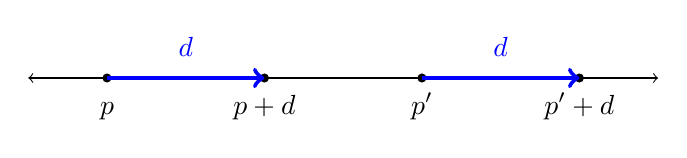
\begin{tikzpicture}
      \draw[<->] (-4,0) -- (4,0);
      \filldraw (-3,0) circle [radius=0.05];
      \draw (-3,-0.65) node[anchor=south] {$p$};
      \filldraw (-1,0) circle [radius=0.05];
      \draw (-1,-0.65) node[anchor=south] {$p + d$};
      \filldraw (+1,0) circle [radius=0.05];
      \draw (+1,-0.65) node[anchor=south] {$p'$};
      \filldraw (+3,0) circle [radius=0.05];
      \draw (+3,-0.65) node[anchor=south] {$p' + d$};
      \draw[->,ultra thick,blue] (-3,0) -- (-1,0);
      \draw[->,ultra thick,blue] (1,0) -- (3,0);
      \draw (-2,0.4) node[blue] {$d$};
      \draw (+2,0.4) node[blue] {$d$};
   \end{tikzpicture}
\end{center}

\noindent Sliding a displacement from one location to another does not cause
the displacement to lose its identity.

\begin{definition}[Scaling]
   For any displacement $d$, a real number $r$ \emph{scales} $d$ as
   by multiplication to form another displacement $e = r d =
   d r$, so that $r$ is the ratio of the length of $e$ to the
   length of $d$.
   \begin{itemize}
      \item If $r = 0$, then $e$ is the \emph{null displacement}
         $0$, which has neither length nor direction.
      \item If $r < 0$, then $e$ points in the direction opposite to that
         of $d$.
      \item If $r = 1$, then $e = d$.
      \item We define the symbol ``$\:-$'' for the displacement such that if $r
         = -1$, then $e = -d$.
   \end{itemize}
   Scaling the displacement, the real number is in this context called a
   \emph{scalar}.
\label{def:scalar}
\end{definition}

\noindent Definition~\ref{def:scalar} provides the fundamental basis for our
geometric intuition about the nature of the reals. The following example
illustrates the definition by way of $-\sqrt{2}$, an irrational
scalar.\footnote{%
   When the proof for the irrationality of $\sqrt{2}$ was recognized by the
   ancient Greeks, the proof appears to have caused some controversy. At least
   for a time, the Greeks preferred to imagine that a unit length could be
   scaled only by a rational number, the ratio of two integers. The idea is
   that, for an integer $n$, a unit length could be subdivided into $n$ equal
   subunits. Then an integer number $m$ of subunits could be stacked end-to-end
   in order to make, by the appropriate choice of $n$ and $m$, an overall
   length of any desired magnitude. That is equivalent to multiplying the
   original unit length by the rational number $m/n$. The side of a square,
   chosen as the unit length, would need to be scaled by $\sqrt{2}$ in order to
   equal the length of the diagonal. For $\sqrt{2}$ to be irrational means that
   there exists no $n$ that can subdivide the side in such a way that $m$
   subunits would equal the length of the diagonal. The problem for us is that
   although the rational scaling is easy to visualize, we must somehow
   comfortably visualize an irrational scaling.  In its decimal representation,
   an irrational number does not repeat, but by truncating or rounding the
   decimal expression at any desired level of accuracy, we may approximate the
   irrational number by a rational number.  We can get an idea of the
   irrational scaling by thinking of a rationally scaled length that converges
   to the right, irrationally scaled length as we extend the decimal expression
   further and further out. The intuitive, geometric idea of convergence comes
   from recognizing that, with each successive digit in the decimal expression,
   the correction to the length becomes about ten times smaller than the
   previous correction.
}

\begin{center}
   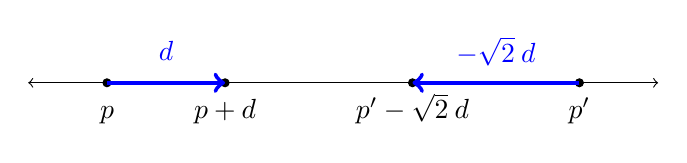
\begin{tikzpicture}
      \draw[<->] (-4,0) -- (4,0);
      \filldraw (-3.0,0) circle [radius=0.05];
      \filldraw (-1.5,0) circle [radius=0.05];
      \filldraw (+0.88,0) circle [radius=0.05];
      \filldraw (+3.00,0) circle [radius=0.05];
      \draw (-3.0,-0.65) node[anchor=south] {$p$};
      \draw (-1.5,-0.65) node[anchor=south] {$p + d$};
      \draw (+3.00,-0.65) node[anchor=south] {$p'$};
      \draw (+0.88,-0.65) node[anchor=south] {$p' - \sqrt{2} \: d$};
      \draw[->,ultra thick,blue] (-3.00,0) -- (-1.50,0);
      \draw[->,ultra thick,blue] (+3.00,0) -- (+0.88,0);
      \draw (-2.25,0.4) node[blue] {$d$};
      \draw (+1.94,0.4) node[blue] {$-\sqrt{2} \: d$};
   \end{tikzpicture}
\end{center}

\noindent The negative sign in $-\sqrt{2}$ causes $-\sqrt{2} \: d$ to point in
the direction opposite to that of $d$. The size of $\sqrt{2}$ causes $-\sqrt{2}
\: d$ to be a bit more than $1.41$ times the length of $d$.

\begin{definition}
   For any two displacements $d$ and $e$ on a line, we define a sense of the
   symbol ``$\:+$'' such that the sum is written $f = d + e$, and, when the
   displacements be visualized with arrows, if the head of $d$ be placed at the
   tail of $e$, and if the tail of $f$ be placed at the tail of $d$, then the
   head of $f$ is located at the head of $e$.
\label{def:head-to-tail}
\end{definition}

\noindent Just as the ordinary operation of addition combines a pair of numbers
and produces a number, so, too, the operation defined above combines a pair of
displacements and produces another displacement. We saw that the difference of
two points is a displacement and that the sum of a point and a displacement is
another point. For the sum of two displacements to be another displacement
makes displacements, considered by themselves under addition, like ordinary
numbers. In fact, we shall see below that the relationship is deep, and we can
sensibly define a one-to-one relationship between displacements along the line
and real numbers.  The illustration below shows that, according to
Definition~\ref{def:head-to-tail}, displacements add together in a
\emph{head-to-tail} manner. In the sum $d + e$, the head of the augend $d$ is
attached to the tail of the addend $e$, and the sum points from the tail of the
augend to the head of the addend.\footnote{%
   The augend is that which is to be augmented., and the addend is that which
   is to be added.%
}

\begin{center}
   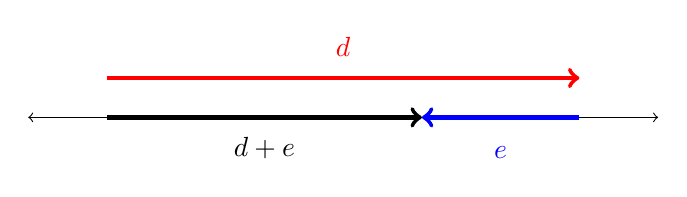
\begin{tikzpicture}
      \draw[<->] (-4,0) -- (4,0);
      \draw[->,ultra thick,red] (-3,0.5) -- (3,0.5);
      \draw[->,ultra thick,blue] (+3,0.0) -- (1,0.0);
      \draw[->,ultra thick] (-3,0.0) -- (1,0.0);
      \draw (0,0.9) node[red] {$d$};
      \draw (+2,-0.65) node[anchor=south,blue] {$e$};
      \draw (-1,-0.65) node[anchor=south] {$d + e$};
   \end{tikzpicture}
\end{center}

\begin{theorem}
   For any displacement $d$ on a line and for any two real numbers $r$ and $s$,
   $r d + s d = [r + s] d$.
\label{theorem:disp-dist}
\end{theorem}

\begin{definition}
   For any two displacements $d$ and $e$ on a line $L$, we define the symbol
   ``$\:-$'' for the difference of displacements such that $e - d = e +
   [-d\:]$.
\label{def:disp-sub}
\end{definition}

\begin{theorem}
   For any sum $f = d + e$ of displacements on a line $L$, $d = f - e$, and $e
   = f - d$.
   \begin{proof}
      By hypothesis we have $f = d + e$. By Definition~\ref{def:head-to-tail},
      the displacements may be arranged head-to-tail.
      \begin{center}
         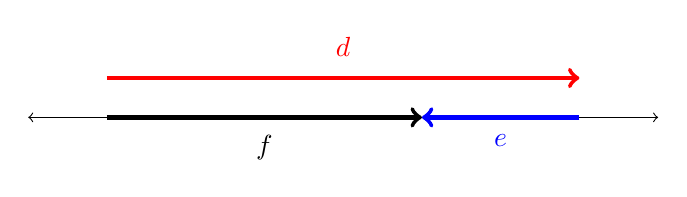
\begin{tikzpicture}
            \draw[<->] (-4,0) -- (4,0);
            \draw[->,ultra thick,red] (-3,0.5) -- (3,0.5);
            \draw[->,ultra thick,blue] (+3,0.0) -- (1,0.0);
            \draw[->,ultra thick] (-3,0.0) -- (1,0.0);
            \draw (0,0.9) node[red] {$d$};
            \draw (+2,-0.1) node[anchor=north,blue] {$e$};
            \draw (-1,-0.1) node[anchor=north] {$f$};
         \end{tikzpicture}
      \end{center}
      By Definition~\ref{def:scalar}, $-e$ has the same length as $e$ does and
      so will fit in its place, though with head and tail reversed.
      \begin{center}
         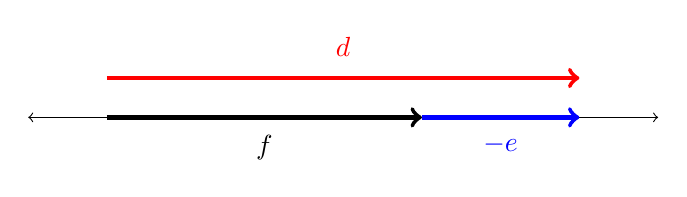
\begin{tikzpicture}
            \draw[<->] (-4,0) -- (4,0);
            \draw[->,ultra thick,red] (-3,0.5) -- (3,0.5);
            \draw[<-,ultra thick,blue] (+3,0.0) -- (1,0.0);
            \draw[->,ultra thick] (-3,0.0) -- (1,0.0);
            \draw (0,0.9) node[red] {$d$};
            \draw (+2,-0.1) node[anchor=north,blue] {$-e$};
            \draw (-1,-0.1) node[anchor=north] {$f$};
         \end{tikzpicture}
      \end{center}
      By Definition~\ref{def:head-to-tail}, $d = f + [-e\:]$.  By
      Definition~\ref{def:disp-sub}, $d = f - e$.  The same process may be
      applied to reverse $d$ (instead of $e\:$) in order to derive $e = f - d$.
   \end{proof}
\end{theorem}

\begin{definition}
   A \emph{Cartesian coordinate system} $\kappa$ on a line is a bijection from
   the real numbers to the points on the line, such that for any real number
   $r$, there is on the line a point $\kappa(r) = \kappa(0) + r \:
   \mathrm{u}_\kappa$, where $r$ is \emph{the coordinate}; the point
   $\kappa(0)$ is the \emph{origin}; and $\mathrm{u}_\kappa = \kappa(1) -
   \kappa(0)$ is the \emph{unit displacement} under $\kappa$.
\end{definition}

\noindent The unit displacement $\mathrm{u}_\kappa$ can be visualized as follows:

\begin{center}
   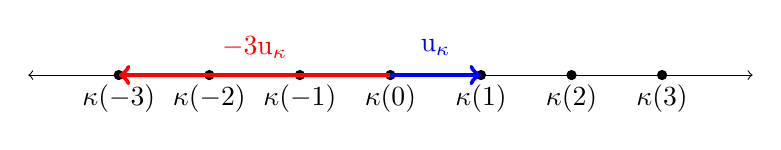
\begin{tikzpicture}[scale=1.15]
      \draw[<->] (-4,0) -- (4,0);
      \filldraw (-3,0) circle [radius=0.05] node[anchor=north] {$\kappa(-3)$};
      \filldraw (-2,0) circle [radius=0.05] node[anchor=north] {$\kappa(-2)$};
      \filldraw (-1,0) circle [radius=0.05] node[anchor=north] {$\kappa(-1)$};
      \filldraw (+0,0) circle [radius=0.05] node[anchor=north] {$\kappa(0)$};
      \filldraw (+1,0) circle [radius=0.05] node[anchor=north] {$\kappa(1)$};
      \filldraw (+2,0) circle [radius=0.05] node[anchor=north] {$\kappa(2)$};
      \filldraw (+3,0) circle [radius=0.05] node[anchor=north] {$\kappa(3)$};
      \draw[->,ultra thick,blue] (0,0) -- (1,0);
      \draw[->,ultra thick,red] (0,0) -- (-3,0);
      \draw (+0.5,0.3) node[blue] {$\mathrm{u}_\kappa$};
      \draw (-1.5,0.3) node[red] {$-3\mathrm{u}_\kappa$};
   \end{tikzpicture}
\end{center}

\noindent When there is only one coordinate system under consideration, we draw
the coordinate line as follows:

\begin{center}
   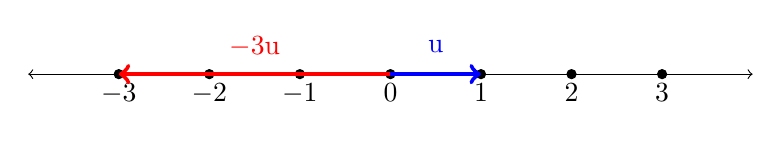
\begin{tikzpicture}[scale=1.15]
      \draw[<->] (-4,0) -- (4,0);
      \filldraw (-3,0) circle [radius=0.05] node[anchor=north] {$-3$};
      \filldraw (-2,0) circle [radius=0.05] node[anchor=north] {$-2$};
      \filldraw (-1,0) circle [radius=0.05] node[anchor=north] {$-1$};
      \filldraw (+0,0) circle [radius=0.05] node[anchor=north] {$0$};
      \filldraw (+1,0) circle [radius=0.05] node[anchor=north] {$1$};
      \filldraw (+2,0) circle [radius=0.05] node[anchor=north] {$2$};
      \filldraw (+3,0) circle [radius=0.05] node[anchor=north] {$3$};
      \draw[->,ultra thick,blue] (0,0) -- (1,0);
      \draw[->,ultra thick,red] (0,0) -- (-3,0);
      \draw (+0.5,0.3) node[blue] {$\mathrm{u}$};
      \draw (-1.5,0.3) node[red] {$-3\mathrm{u}$};
   \end{tikzpicture}
\end{center}

\begin{theorem}
   For a Cartesian coordinate system $\kappa$ on a line $L$, and for any two
   real numbers $r$ and $s$, the displacement between the corresponding points
   is $\kappa(s) - \kappa(r) = [s - r] \mathrm{u}_\kappa$.
\label{theorem:displacement}
\end{theorem}

\noindent Theorem~\ref{theorem:displacement} expresses the relationship between
a displacement of the first kind (the difference $s - r$) and a displacement of
the second kind (the abstract, geometric displacement $\kappa(s) - \kappa(r)$).

\subsection{Order}

\begin{definition}
   For a Cartesian coordinate system $\kappa$ on a line $L$, the \emph{positive
   direction} on $L$ is the direction of $\mathrm{u}_\kappa$. The
   \emph{negative direction} on $L$ is the direction of $-\mathrm{u}_\kappa$.
\end{definition}

\noindent When there is a single coordinate line, it is almost always drawn
horizontally with the positive direction to the right.

The set $S_{>a} = \{r \in R : r > a\}$ is depicted on the line as a positively
directed ray emanating from the point labeled $a$ (or labeled $\kappa(a)$ when
the coordinate system is made explicit). Because $a \notin S_{>a}$, an open
circle is placed around the point corresponding to $a$.

\begin{center}
   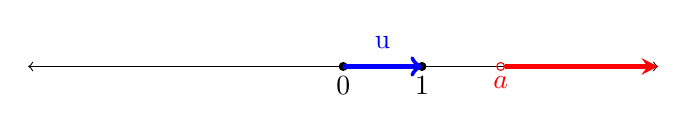
\begin{tikzpicture}
      \draw[<->] (-4,0) -- (4,0);
      \filldraw (+0,0) circle [radius=0.05] node[anchor=north] {$0$};
      \filldraw (+1,0) circle [radius=0.05] node[anchor=north] {$1$};
      \draw[red] (+2,0) circle [radius=0.05] node[anchor=north] {$a$};
      \draw[->,ultra thick,blue] (0,0) -- (1,0);
      \draw[->,>=stealth,ultra thick,red] (+2.05,0) -- (4,0);
      \draw (+0.5,0.3) node[blue] {$\mathrm{u}$};
   \end{tikzpicture}
\end{center}

\subsection{Distance}

\subsection{Exercises}

\begin{exercise}
   Draw a diagram like the one used to illustrate
   Definition~\ref{def:head-to-tail}, but reverse the order of the addition.
   That is, show geometrically that the same result $f$ obtains by adding the
   displacements head-to-tail in the order $e + d$.
\end{exercise}

\begin{exercise}
   Pick any two displacements $d$ and $e$ that point in the same direction
   along a line. Draw a diagram showing that their sum is the same, regardless
   of the order in which they are added.
\end{exercise}

\begin{exercise}
   Pick two displacements $d$ and $e$ that point in the same direction along a
   line, and let $d$ be longer than $e$. Draw a diagram showing that their
   difference depends on the order in which they are subtracted.
\end{exercise}

\begin{exercise}
   (Optional, difficult.) Prove Theorem~\ref{theorem:disp-dist}.
   \begin{solution}
      There are three cases to consider.
      \begin{enumerate}
         \item Either $r = 0$ or $s = 0$ (or $r = s = 0$). Suppose that $s =
            0$. By Definition~\ref{def:scalar}, $s d = 0 d = 0$, which has zero
            length. By Definition~\ref{def:head-to-tail}, $r d + s d = r d$
            because the head and the tail of $s d$ are at the same point.
            Finally, we write $r d + s d = [r + 0] d = [r + s] d$. The same
            result obtains by a similar argument on the supposition that $r =
            0$.
         \item Either both $r < 0$ and $s < 0$ or both $r > 0$ and $s > 0$;
            that is, $r$ and $s$ have the same sign. In this case, by
            Definition~\ref{def:scalar}, both $r d$ and $s d$ point in the same
            direction. Then by Definition~\ref{def:head-to-tail}, the length of
            $r d + s d$ is the sum of the lengths of $r d$ and $s d$.
            \begin{center}
               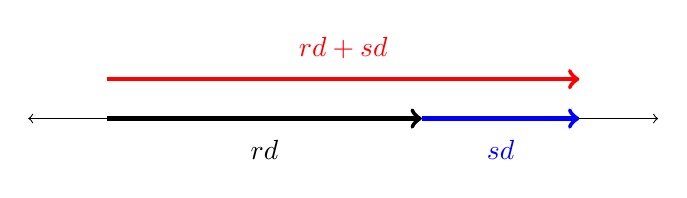
\begin{tikzpicture}
                  \draw[<->] (-4,0) -- (4,0);
                  \draw[->,ultra thick,red] (-3,0.5) -- (3,0.5);
                  \draw[<-,ultra thick,blue] (+3,0.0) -- (1,0.0);
                  \draw[->,ultra thick] (-3,0.0) -- (1,0.0);
                  \draw (0,0.9) node[red] {$r d + s d$};
                  \draw (+2,-0.65) node[anchor=south,blue] {$s d$};
                  \draw (-1,-0.65) node[anchor=south] {$r d$};
               \end{tikzpicture}
            \end{center}
            By Definition~\ref{def:scalar}, the ratio of the length of $r d$ to
            the length of $d$ is $r$; the ratio of the length of $s d$ to the
            length of $d$ is $s$; and, because the length of the sum of the
            displacements is in this case the sum of the lengths of the
            displacements, the ratio of the length of $r d + s d$ to the length
            of $d$ is $|r + s|$.  The sign of $r + s$ is the same as the sign
            of $r$ and $s$. By Definition~\ref{def:head-to-tail}, $r d + s d$
            points in the same direction as $r d$ and $s d$, and, by
            Definition~\ref{def:scalar}, the sign of the scalar directs the
            product; therefore $r d + s d = [r + s] d$.
         \item Either both $r < 0$ and $s > 0$ or both $r > 0$ and $s < 0$;
            that is, $r$ and $s$ have opposite signs. In this case, by
            Definition~\ref{def:scalar}, $r d$ and $s d$ point in opposite
            directions. There are three subcases to consider.
            \begin{enumerate}
               \item Suppose that $|r| = |s|$ so that $r d$ is the same length
                  as $s d$. Then by Definition~\ref{def:head-to-tail}, the
                  length of $r d + s d$ is zero. We have by hypothesis,
                  however, that $r + s = 0$, because $r$ and $s$ are of
                  opposite signs but equal magnitude. So we can can write that
                  $r d + s d = 0 d = [r + s] d$.
               \item Suppose that $|r| > |s|$ so that $r d$ is longer than $s
                  d$. Then by Definition~\ref{def:head-to-tail}, the length of
                  $r d + s d$ is the length of $r d$ minus the length of $s d$.
                  \begin{center}
                     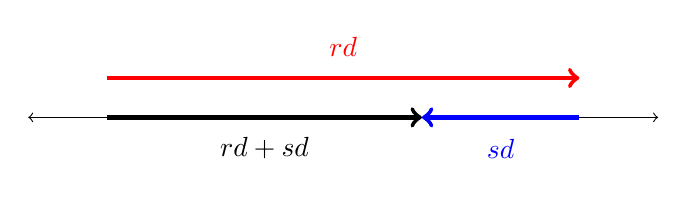
\begin{tikzpicture}
                        \draw[<->] (-4,0) -- (4,0);
                        \draw[->,ultra thick,red] (-3,0.5) -- (3,0.5);
                        \draw[->,ultra thick,blue] (+3,0.0) -- (1,0.0);
                        \draw[->,ultra thick] (-3,0.0) -- (1,0.0);
                        \draw (0,0.9) node[red] {$r d$};
                        \draw (+2,-0.65) node[anchor=south,blue] {$s d$};
                        \draw (-1,-0.65) node[anchor=south] {$r d + s
                        d$};
                     \end{tikzpicture}
                  \end{center}
                  By Definition~\ref{def:scalar}, the ratio of the length of $r
                  d$ to the length of $d$ is $r$; the ratio of the length of $s
                  d$ to the length of $d$ is $s$; and, because the length of
                  the sum of the displacements is in this case the difference
                  of the lengths of the displacements, the ratio of the length
                  of $r d + s d$ to the length of $d$ is $|r| - |s|$. Because
                  $|r| > |s|$ and because $r$ and $s$ have opposite signs, $|r|
                  - |s| = |r + s|$.  The sign of $r + s$ is the same as the
                  sign of $r$.  By Definition~\ref{def:head-to-tail}, $r d + s
                  d$ points in the same direction as $r d$, and, by
                  Definition~\ref{def:scalar}, the sign of the scalar directs
                  the product; therefore $r d + s d = [r + s] d$.
               \item Suppose that $|s| > |r|$ so that $s d$ is longer than $r
                  d$. Then by Definition~\ref{def:head-to-tail}, the length of
                  $r d + s d$ is the length of $s d$ minus the length of $r d$.
                  \begin{center}
                     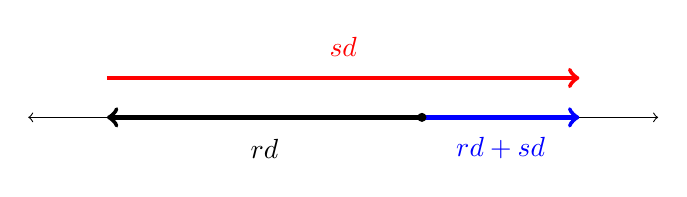
\begin{tikzpicture}
                        \draw[<->] (-4,0) -- (4,0);
                        \draw[->,ultra thick,red] (-3,0.5) -- (3,0.5);
                        \draw[<-,ultra thick,blue] (+3,0.0) -- (1,0.0);
                        \draw[<-,ultra thick] (-3,0.0) -- (1,0.0);
                        \filldraw (1,0) circle [radius=0.05];
                        \draw (0,0.9) node[red] {$s d$};
                        \draw (+2,-0.65) node[anchor=south,blue] {$r d + s d$};
                        \draw (-1,-0.65) node[anchor=south] {$r d$};
                     \end{tikzpicture}
                  \end{center}
                  By Definition~\ref{def:scalar}, the ratio of the length of $r
                  d$ to the length of $d$ is $r$; the ratio of the length of $s
                  d$ to the length of $d$ is $s$; and, because the length of
                  the sum of the displacements is in this case the difference
                  of the lengths of the displacements, the ratio of the length
                  of $r d + s d$ to the length of $d$ is $|s| - |r|$. Because
                  $|s| > |r|$ and because $r$ and $s$ have opposite signs, $|s|
                  - |r| = |s + r| = |r + s|$.  The sign of $r + s$ is the same
                  as the sign of $s$.  By Definition~\ref{def:head-to-tail}, $r
                  d + s d$ points in the same direction as $s d$, and, by
                  Definition~\ref{def:scalar}, the sign of the scalar directs
                  the product; therefore $r d + s d = [r + s] d$.
            \end{enumerate}
      \end{enumerate}
   \end{solution}
\end{exercise}

\begin{exercise}
   Prove Theorem~\ref{theorem:displacement}. Avoid algebraic rearrangement of
   any expression involving points.  Hint: Draw a diagram with points
   $\kappa(0)$, $\kappa(r)$, and $\kappa(s)$ on the line. Use
   Definition~\ref{def:head-to-tail} and Theorem~\ref{theorem:disp-dist}.
\end{exercise}

